\documentclass{scrartcl}
\usepackage[T1]{fontenc}
\usepackage{amsmath}
\usepackage{amsthm}
\usepackage[utf8]{inputenc}
\usepackage{amssymb}
\usepackage{lmodern}
\usepackage{blindtext}
\usepackage{tikz}
\usepackage{listings}
\usepackage{url}
\usepackage{subfigure}
\usepackage{float}

\newtheoremstyle{my_th_style}%
	{3pt}%		// space above
	{3pt}%		// space below
	{}%		// body font
	{}%		// indent amount
	{\bfseries}%	// theorem head font
	{}%		// punctuation after theorem head
	{\newline}%	// space after theorem head
	{}%		// theorem head spec
\theoremstyle{my_th_style}
\newtheorem{defi}{Definition}[section]
\newtheorem{bsp}{Beispiel}[section]
\newtheorem{satz}{Satz}[section]
\newtheorem{kor}{Korallar}[section]
\newtheorem{bew}{Beweis}
\newtheorem{lem}{Lemma}
\usepackage{selinput}% Eingabecodierung automatisch ermitteln …
\SelectInputMappings{% … siehe <http://ctan.org/pkg/selinput>
  adieresis={ä},
  germandbls={ß},
}
\usepackage[ngerman]{babel}% Das Beispieldokument ist in Deutsch,
                % daher wird mit Hilfe des babel-Pakets
                % über Option ngerman auf deutsche Begriffe
                % und gleichzeitig Trennmuster nach den
                % aktuellen Rechtschreiberegeln umgeschaltet.
                % Alternativen und weitere Sprachen sind
                % verfügbar (siehe <http://ctan.org/pkg/babel>).
\begin{document}
% ----------------------------------------------------------------------------
% Titel (erst nach \begin{document}, damit babel bereits voll aktiv ist:
\subject{Projektarbeit}% optional
\title{Big Data}% obligatorisch
\author{Matthias Körschens, Kevin Reinke}% obligatorisch
\date{\today}% sinnvoll
\maketitle% verwendet die zuvor gemachte Angaben zur Gestaltung eines Titels
% ----------------------------------------------------------------------------
% Inhaltsverzeichnis:
\tableofcontents
% ----------------------------------------------------------------------------
% Gliederung und Text:
\begingroup
\let\cleardoublepage\relax
\section{Einleitung}
Ziel der Projektarbeit war es, die im Rahmen der Vorlesung \glqq Big Data\grqq erworbenen Fähigkeiten praktisch umzusetzten. Hierfür konnten wir einen Amazonreview-Datensatz der Stanford University nutzen. Ein Dank geht an dieser Stelle an Julian McAuley, der so freundlich war uns diesen Datensatz auf Nachfrage zur Verfügung zu stellen. Zur Bearbeitung der Daten haben wir Apache Spark, sowie den Clusterrechner der FSU-Jena benutzt. Fragestellung unserer Bearbeitung war das erkennen von Muster in den Daten. Im speziellen haben wir uns auf die Verteilung der Reviews und das Bewertungsverhalten der Nutzer konzentriert.
\section{Datensatz}
Der in dieser Arbeit verwendete Datensatz besteht aus Reviews des Onlinehändlers Amazon aus der Zeitspanne von Mai 1996 bis Juni 2014. Es wird hier ein spezieller Teildatensatz verwendet, welcher lediglich Reviews aus der Kategorie Elektronik enthält. Dieser hat mit 7,8 Millionen Reviews von etwa 4,2 Millionen Nutzern eine Größe von 4,7 Gigabyte. Er ist vollständig im JSON-Format gehalten. Ein Beispielreview ist nachfolgend dargestellt:

\begin{lstlisting}[breaklines=true]
{ 
  "reviewerID": "A2SUAM1J3GNN3B", 
  "asin": "0000013714", 
  "reviewerName": "J. McDonald", 
  "helpful": [2, 3], 
  "reviewText": "I bought this for my husband who plays the piano. He is having a wonderful time playing these old hymns. The music is at times hard to read because we think the book was published for singing from more than playing from. Great purchase though!", 
  "overall": 5.0, 
  "summary": "Heavenly Highway Hymns", 
  "unixReviewTime": 1252800000, 
  "reviewTime": "09 13, 2009" 
}
\end{lstlisting}

Die Datensätze bestehen aus der ID des Reviewers (reviewerID), der Produkt-ID (asin), dem Namen des Reviewers (reviewerName), einer Liste mit zwei numerischen Werten, die die hilfreich-Bewertungen repräsentieren (helpful), dem Inhalt der Review (reviewText), der Produktbewertung (overall), der Überschrift bzw. Zusammenfassung des Reviews (summary), dem Datum der Review (reviewTime) und dem Datum im Unix-Format (unixReviewTime). Aufgrund der gegebenen Reviewer-ID lassen sich so auch neben den Reviews Rückschlüsse über die einzelnen Reviewer ziehen.\\
Der Datensatz ist verfügbar unter \url{http://jmcauley.ucsd.edu/data/amazon/}.
\section{Strukturen}
\subsection{Verteilung der Reviews}
Eine Fragestellung ist die Verteilung der Reviews auf die Nutzer. Hierfür haben wir die Reviews mit gleicher ReviewerID aufaggregiert und die Anzahl der Reviews, die ein Nutzer abgegeben hat, dem Nutzer zugeordnet. Dabei ist aufgefallen, dass die erfassten Nutzer eher wenig bewerten. Beispielsweisen gibt es etwa 2,88 von 4,2 Millionen Nutzern die nur ein einziges Review abgaben. In Abbildung 0.1 ist die Anzahl der Nutzer, die eine spezifische Anzahl an Reviews abgegeben haben, dargestellt. Für eine bessere Visualisierung wurden beide Achsen logarithmiert. 
\begin{figure}[H]
\centering
    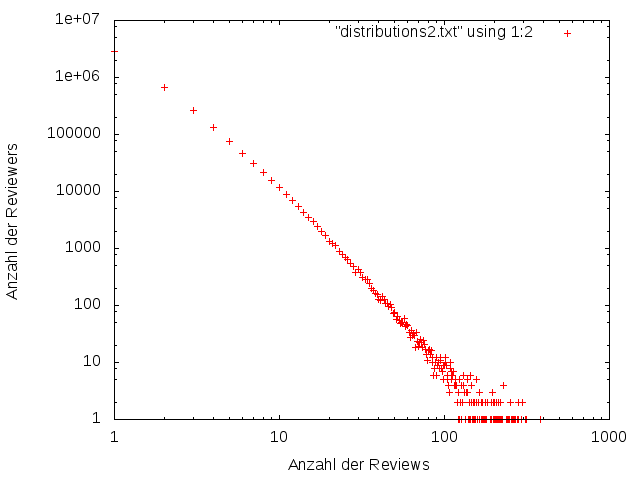
\includegraphics[width=0.8\textwidth]{bild.png}
    \caption{Reviewverteilung}
\end{figure}
Der Zusammenhang schein exponentiell zu sein. Da ferner die Gruppen nach der Anzahl der Reviews sortiert wurden, erinnert dies an das Zipfsche Gesetzt aus der Linguistik.

\subsection{Reviewerverhalten bei steigener Reviewanzahl}
Zunächst haben wir die Gruppierung der Nutzer nach ihrer Anzahl an Reviews beibehalten und untersucht, ob sich diese Gruppen unterschiedliches verhalten aufzeigen. Innerhalb einer Gruppe wurden für die Merkmale die Gruppendurchschnitte errechnet. Die Merkmale und ihr Zusammenhang in Abhängigkeit der Reviewanzahl sind in den Grafiken im Anhang dargestellt.\\
Wie im vorigen Abschnitt angesprochen überwiegen die Nutzer mit wenig Reviews. Daher ist die Durchschnittsbildung über die Merkmale bei den Gruppen mit wenig Reviews(mehr Reviewer je Gruppe) stabiler. Für Gruppen mit mehr 100 Reviews, kann es unter Umständen sein, dass diese nur aus einen einzigen Reviewer besteht. Dies zeigt sich in der starken Streuung der vier Grafen mit zunehmender Reviewanzahl. Aus diesen Grund wurde die Achse der Reviewanzahl logarithmiert, um die relevanteren Gruppen in den Fokus zu rücken. Auch wenn der Durchschnitt für einige Gruppen nicht sehr aussagekräftig ist, so lassen sich dennoch deutliche Zusammenhänge erkennen. Nutzer die mehrere Reviews verfassen, schreiben ausführlichere Bewertungstexte und werden von anderen Nutzern als hilfreicher eingestuft. Ebenso scheinen sie Produkte leicht besser zu bewerten.

\subsection{Textlänge und Produktbewertung}
Ein interessanter Zusammenhang hat sich bei der Beziehung zwischen der Textlänge des Reviews und der Produktbewertung gezeigt. Die Textlänge haben wir im folgenden nach Zeichen- und  Wortanzahl untersucht. Dabei wurden alle Reviews mit gleicher Länge zusammengruppiert und über diese Gruppen die durchschnittlichen Produktbewertungen bestimmt. 
\begin{figure}[H]
\centering
    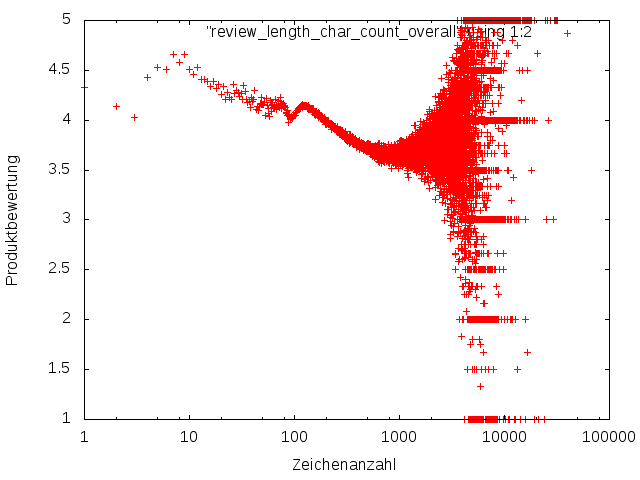
\includegraphics[width=0.7\textwidth]{_results/char_rating.png}
\end{figure}
\begin{figure}[H]
\centering
    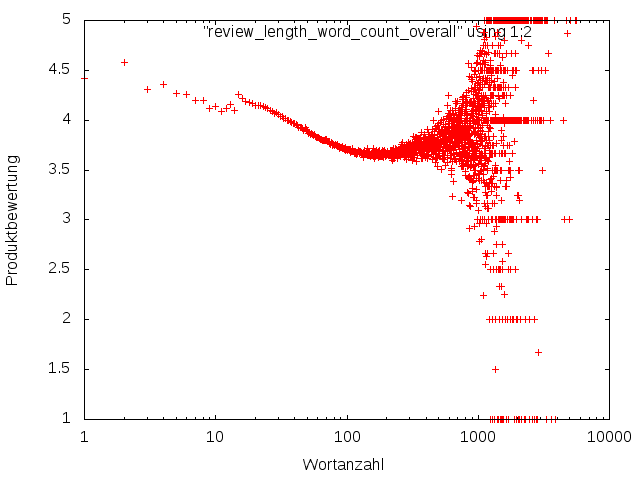
\includegraphics[width=0.7\textwidth]{_results/word_rating.png}

\end{figure}
Hier sind die Produktbewertungen mit wenig Wörtern anfänglich zwischen 4,0 und 4,5. Mit zunehmender Textlänge bis etwa 180 Wörtern fällt die Bewertung auf 3,6 erholt sich danach aber wieder leicht. Ab 1000 Wörtern sind zuverlässige Aussgen wieder nicht mehr möglich, da die Gruppen zu klein werden.

\section{Cluster}
Um die Nutzer untereinander in Beziehung zu setzten, mussten wir jeden Reviewer ein Merkmalsvektor zuordnen. Diesen haben wir über arithmetische Mittelung der vom Nutzer abgegebenen Reviews bestimmt. Die Merkmale sind dabei:
\begin{itemize}
\item Wortanzahl des Bewertungstextes
\item Zeichenanzahl des Bewertungstextes
\item Zeitstempel des Reviews
\item Zeichenanzahl des Reviewtitels
\item wie hilfreich das Review war prozentual
\item wieviele das Review ingesamt nützlich fanden
\item Produktbewertung
\end{itemize}

Agglomeratives Clusterverfahren, welches ein Distanzmaß zwischen allen Reviewern benutzt, haben wir verworfen, da hierfür ein quadratischer Aufwand in Anzahl der Reviewer anfallen würde.\\
Als ersten Schritt haben wir die Daten mit der Hauptachsentransformation bearbeitet. Hierfür wurde die Bibliothek pyspark.mllib.feature benutzt. Leider hat sie als Rückgabewerte keine Transformationsmatrix oder Eigenwerte geliefert, sodass keine Aussagen über die Einflüsse der einzelnen Merkmale möglich waren. Im Anschluss wurden die Daten mit dem K-means Algorithmus der Bibliothek pyspark.mllib.cluserting gruppiert. Der Algorithmus wurde mit 10 zufälligen Startkonfigurationen ausgeführt und über die entstandenen Merkmalsverktoren der Cluster gemittelt. Als Clusteranzahl haben wir $k=2,44$ und $65$ gewählt.

\newpage
\section*{Anhang}
\subsection*{Grafiken}
\begin{figure}[H]
   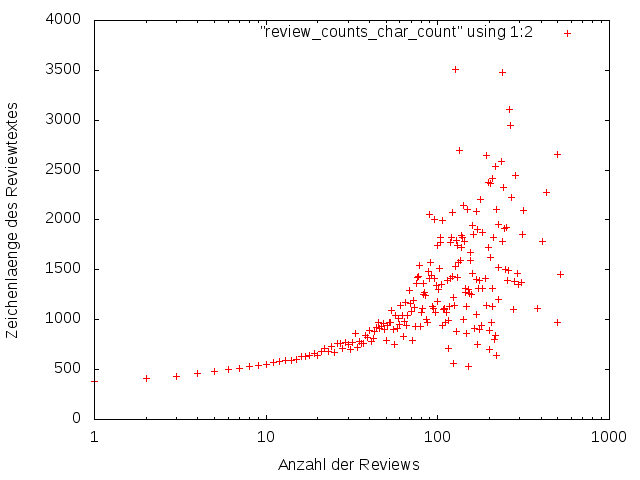
\includegraphics[width=0.8\textwidth]{_results/char_count2.png}
\end{figure}
\begin{figure}[H]
   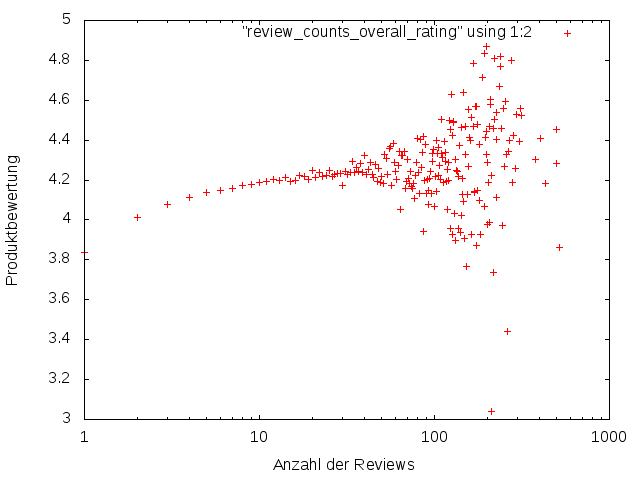
\includegraphics[width=0.8\textwidth]{_results/rating_count.png}
\end{figure}
\begin{figure}[H]
   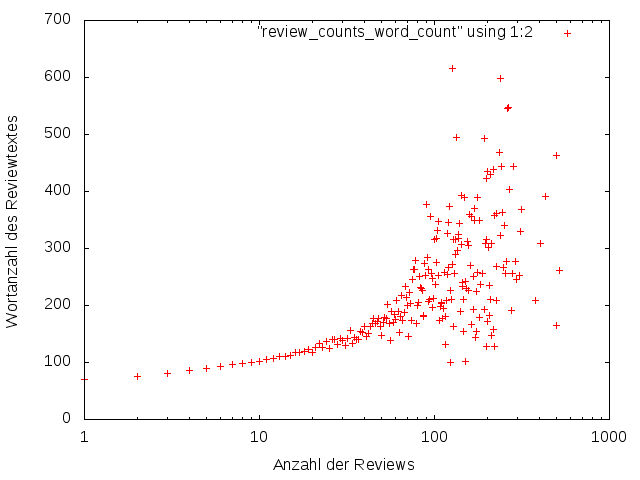
\includegraphics[width=0.8\textwidth]{_results/word_count2.png}
\end{figure}
\begin{figure}[H]
   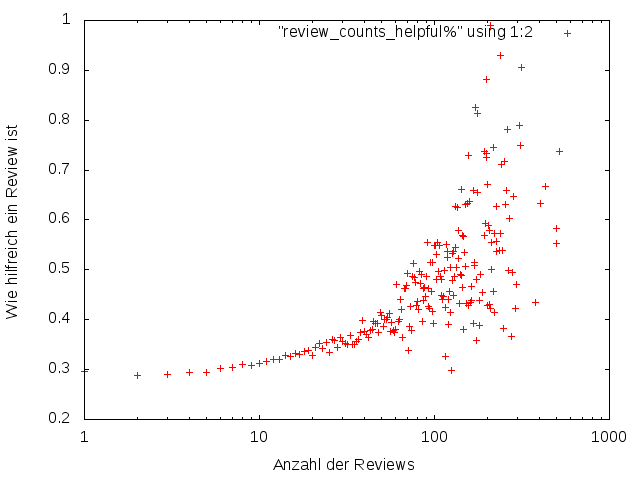
\includegraphics[width=0.8\textwidth]{_results/helpfull_count2.png}
\end{figure}

\newpage
\subsection*{Code}
\underline{run.sh}
\begin{lstlisting}
#!/usr/bin/bash

hdfs dfs -rm -r -f reviews/reviewerReviewsSample
hdfs dfs -rm -r -f reviews/kmeans_model
if [ $# -eq 0 ] 
	then
	/cluster/spark/bin/spark-submit ReviewerReviews.py
	else
	/cluster/spark/bin/spark-submit ReviewerReviews.py -s $1
fi

cat results.txt
\end{lstlisting}
\newpage
\underline{ProcessCluster.py}
\begin{lstlisting}
from pyspark import SparkConf, SparkContext
import json
import argparse
from os import makedirs

#run on cluster
confCluster = SparkConf()
confCluster.setMaster("yarn-client")
confCluster.set("spark.driver.host","frontend")
confCluster.setAppName("AmazonReviews")

sc = SparkContext(conf = confCluster)

result_collection = {}

input_filename = "cluster_output64"

# Read the data in json format line by line
file_data = sc.textFile("reviews/" + input_filename)

file_data = file_data.map(lambda x: x.split(" "))
file_data = file_data.map(lambda x: (int(x[0]), (x[1], float(x[2]), int(x[3]), float(x[4]), int(x[5]), float(x[6]), float(x[7]), float(x[8]), float(x[9]))))

# Reduce each review to vector of usable data elements
#vector_data = file_data.map(lambda d: (d["reviewerID"], (float(d["helpful"][0]) / d["helpful"][1] if d["helpful"][1] != 0 else 0, d["helpful"][1], d["overall"], d["unixReviewTime"], len(d["reviewText"]), len(d["summary"]), len(d["reviewText"].split(" ")), 1)))

# Reduction of reviews per reviewer to vector representing the reviewer
# vectors: (reviewerID, (helpful%, helpful_voted, overall, unixReviewTime, len(reviewText), len(summary), word_count_review_text, reviewCount))

def averages_all_keys(rdd, value_choice_fun):
	trdd = rdd.map(lambda x: (value_choice_fun(x)[0], value_choice_fun(x)[1] + [1]))
	trdd = trdd.reduceByKey(lambda a, b: tuple(a[i] + b[i] for i in range(len(a))))
	trdd = trdd.map(lambda x: (x[0], tuple(val / x[1][-1] for val in x[1][:-1])))
	
	trdd = trdd.sortByKey()

	trdd = trdd.map(lambda x: str(x[0]) + " "  + "".join(" ".join("{}".format(val) for val in x[1])) + "\n")
	#with open("results.txt", "w") as f:
	#	f.write(str(trdd.first()))
	
	return trdd.reduce(lambda a, b: a + b)
	

# Get average char count, word count, overall rating and helpful% per review count
averages = averages_all_keys(file_data, lambda x: (x[0], [x[1][1], x[1][2], x[1][3], x[1][4], x[1][5], x[1][6], x[1][7], x[1][8]])) 

result_collection[input_filename] = averages

# Write results to local disk
try:
	makedirs("results/cluster_results")
except OSError:
	pass

for key in result_collection:
	with open("results/cluster_results/" + key, "w") as f:
		f.write(str(result_collection[key]))

\end{lstlisting}
\newpage
\underline{ReviewerReviews.py}
\begin{lstlisting}
from pyspark import SparkConf, SparkContext
import json
import argparse
from os import makedirs
from pyspark.mllib.linalg import Vectors
from pyspark.mllib.feature import PCA
from pyspark.mllib.clustering import KMeans, KMeansModel

# Program parameters
parser = argparse.ArgumentParser()

parser.add_argument("-s", "--sample", type=float, default=0, help="Use a subset of the data. Has to be a number between 0 and 1, determining the size of the subset to use.")

args = parser.parse_args()

subset_size = args.sample

#run on cluster
confCluster = SparkConf()
confCluster.setMaster("yarn-client")
confCluster.set("spark.driver.host","frontend")
confCluster.setAppName("AmazonReviews")

sc = SparkContext(conf = confCluster)

result_collection = {}

# Read the data in json format line by line
file_data = sc.textFile("reviews/reviews_Electronics.json")
# Each dataset is divided by \n --> parse each line into dict
file_data = file_data.map(json.loads)

# Draw a sample from the dataset
if subset_size != 0:
	file_data = file_data.sample(False, subset_size, 79347234)

# Reduce each review to vector of usable data elements
vector_data = file_data.map(lambda d: (d["reviewerID"], (float(d["helpful"][0]) / d["helpful"][1] if d["helpful"][1] != 0 else 0, d["helpful"][1], d["overall"], d["unixReviewTime"], len(d["reviewText"]), len(d["summary"]), len(d["reviewText"].split(" ")), 1)))

# Reduction of reviews per reviewer to vector representing the reviewer
# vectors: (reviewerID, (helpful%, helpful_voted, overall, unixReviewTime, len(reviewText), len(summary), word_count_review_text, reviewCount))
reviewer_vectors = vector_data.reduceByKey(lambda a, b: tuple(a[i] + b[i] for i in range(len(b))))
reviewer_vectors = reviewer_vectors.map(lambda x: (x[0], [val / x[1][7] for val in x[1][:-1]] + [x[1][-1]]))

def averages_per_key(rdd, value_choice_fun):
	trdd = rdd.map(lambda x: (value_choice_fun(x)[0], value_choice_fun(x)[1] + [1]))
	trdd = trdd.reduceByKey(lambda a, b: tuple(a[i] + b[i] for i in range(len(a))))
	trdd = trdd.map(lambda x: (x[0], tuple(val / x[1][-1] for val in x[1][:-1])))
	
	trdd = trdd.sortByKey()

	trdd = trdd.map(lambda x: tuple("{}\t{}\n".format(x[0], x[1][i]) for i in range(len(x[1]))))
	#with open("results.txt", "w") as f:
	#	f.write(str(trdd.first()))
	
	return trdd.reduce(lambda a, b: tuple(a[i] + b[i] for i in range(len(a))))
	

# Get average char count, word count, overall rating and helpful% per review count
review_counts_cc, review_counts_wc, review_counts_or, review_counts_hp = averages_per_key(reviewer_vectors, lambda x: (x[1][7], [x[1][4], x[1][6],  x[1][2], x[1][0]])) 

result_collection["review_counts_char_count"] = review_counts_cc
result_collection["review_counts_word_count"] = review_counts_wc
result_collection["review_counts_overall_rating"] = review_counts_or
result_collection["review_counts_helpful%"] = review_counts_hp


# Get average overall rating per review length (char count)
review_length_cc, = averages_per_key(reviewer_vectors, lambda x: (x[1][4], [x[1][2]]))
review_length_wc, = averages_per_key(reviewer_vectors, lambda x: (x[1][6], [x[1][2]]))

result_collection["review_length_char_count"] = review_length_cc
result_collection["review_length_word_count"] = review_length_wc

# Conduct PCA
reviewer_vectors_real = reviewer_vectors.map(lambda x: Vectors.dense([val for val in x[1]]))

pca_model = PCA(8).fit(reviewer_vectors_real)
transformed = pca_model.transform(reviewer_vectors_real)

current_best = None
current_best_cost = float("inf")

# Run K-Means
for k in range(2, 70, 7):
	kmeans_model = KMeans.train(transformed, k, maxIterations = 100, runs = 10)

	cost = kmeans_model.computeCost(transformed)

	if cost < current_best_cost:
		current_best_cost = cost
		current_best = kmeans_model

#current_best.save(sc, "reviews/kmeans_model")

predicted = current_best.predict(transformed)

predicted_clusters = predicted.zip(reviewer_vectors.map(lambda x: tuple([x[0]] + [val for val in x[1]])))

predicted_clusters = predicted_clusters.sortByKey()

cluster_output = predicted_clusters.map(lambda x: str(x[0]) + "".join("".join(" {}".format(val)) for val in x[1]) + "\n").reduce(lambda a, b: a + b)

result_collection["cluster_output"] = cluster_output

# Write results to local disk
try:
	makedirs("results")
except OSError:
	pass

for key in result_collection:
	with open("results/" + key, "w") as f:
		f.write(str(result_collection[key]))

\end{lstlisting}
\end{document}



